\documentclass{article}
\usepackage{amsmath}
\usepackage{amssymb}
\usepackage[margin=1in]{geometry}
\usepackage{booktabs}
\usepackage{float}
\usepackage{graphicx}
\usepackage{hyperref}
\usepackage{pdfpages}

\title{Final Project\\Numerical Solutions to PDEs}
\date{9 May 2025}
\author{Connor Emmons and Noah Wells}

\begin{document}
\pagenumbering{gobble}
\maketitle
\begin{figure}[h]
    \centering
    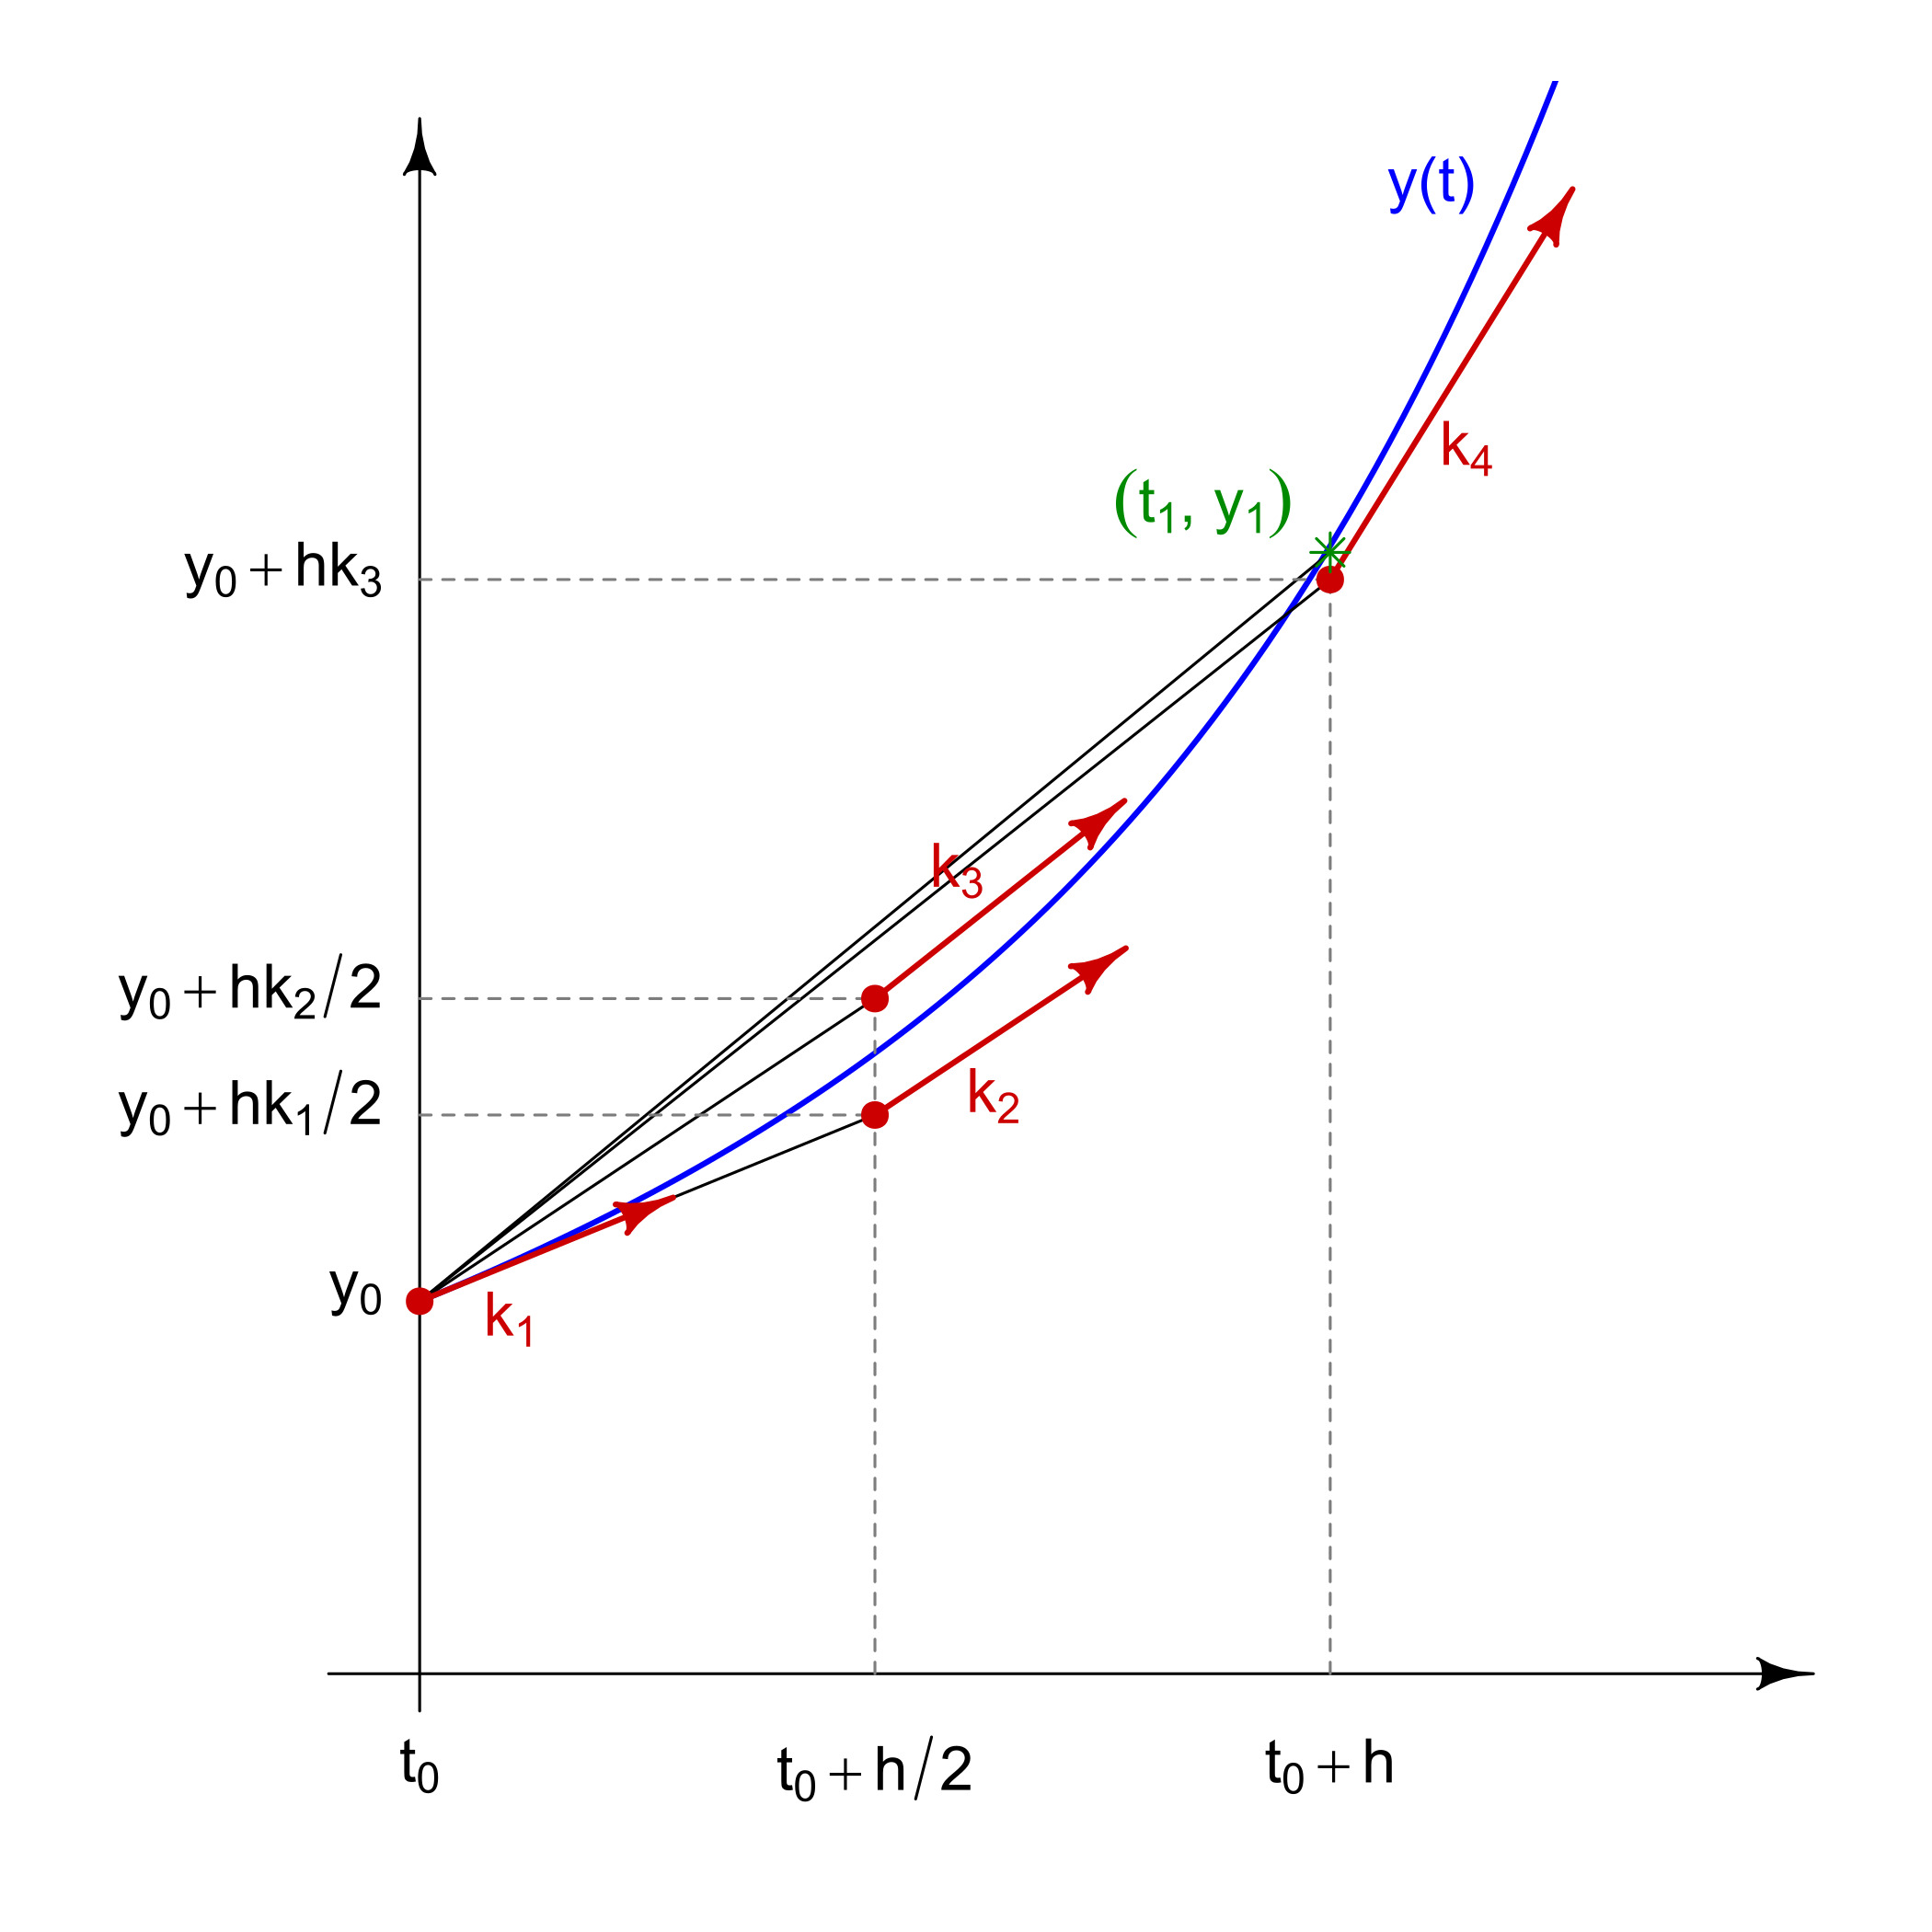
\includegraphics[width=0.8\textwidth]{title.jpg}
\end{figure}
\vfill
\paragraph*{Documentation}
ChatGPT: \url{https://chatgpt.com/share/681eaa76-a3d8-800f-b691-38bc518f0b52}
GitHub: \url{https://github.com/Connor-Lemons/PDE-Final}
\newpage
\pagenumbering{arabic}

\section{Basic Heat Equation}

\subsection*{$u_t = 2u_{xx}\\u(0,t) = u(3,t) = 0\\u(x,0) = \sin(\pi x) + \sin(2\pi x)$}

Using the central difference approximation for second derivatives gives:
\begin{equation}
    \begin{aligned}
        \frac{du}{dt} &= 2\frac{u_{i+1}^n - 2u_i^n + u_{i-1}^n}{\Delta x^2}\\
        u(t_0) &= \sin(\pi x) + \sin(2\pi x)
    \end{aligned}
\end{equation}
Note that the index $i$ relates to the spatial steps and the index $n$ relates to the time steps. The standard RK4 formulation is given as:
\begin{equation}
    \begin{aligned}
        k_1 &= f(t_n, y_n) \\
        k_2 &= f\left(t_n + \frac{h}{2},\, y_n + \frac{h}{2}k_1\right) \\
        k_3 &= f\left(t_n + \frac{h}{2},\, y_n + \frac{h}{2}k_2\right) \\
        k_4 &= f(t_n + h,\, y_n + hk_3) \\
        y_{n+1} &= y_n + \frac{h}{6}\left(k_1 + 2k_2 + 2k_3 + k_4\right)
    \end{aligned}
\end{equation}
Adapting this to the problem at hand gives:
\begin{equation}
    \begin{aligned}
        k_1 &= \alpha \frac{u_{i+1}^{n-1} - 2u_i^{n-1} + u_{i-1}^{n-1}}{\Delta x^2} \\
        k_2 &= \alpha \frac{
            \left(u_{i+1}^{n-1} + \frac{\Delta t}{2}k_1\right)
            - 2\left(u_i^{n-1} + \frac{\Delta t}{2}k_1\right)
            + \left(u_{i-1}^{n-1} + \frac{\Delta t}{2}k_1\right)
        }{\Delta x^2} \\
        k_3 &= \alpha \frac{
            \left(u_{i+1}^{n-1} + \frac{\Delta t}{2}k_2\right)
            - 2\left(u_i^{n-1} + \frac{\Delta t}{2}k_2\right)
            + \left(u_{i-1}^{n-1} + \frac{\Delta t}{2}k_2\right)
        }{\Delta x^2} \\
        k_4 &= \alpha \frac{
            \left(u_{i+1}^{n-1} + \Delta t\, k_3\right)
            - 2\left(u_i^{n-1} + \Delta t\, k_3\right)
            + \left(u_{i-1}^{n-1} + \Delta t\, k_3\right)
        }{\Delta x^2} \\
        u_i^{n} &= u_i^{n-1} + \frac{\Delta t}{6} \left( k_1 + 2k_2 + 2k_3 + k_4 \right)
    \end{aligned}
\end{equation}
An example of the numerical solution plotted against the analytical solution is shown below. In order to view the full animation, please run the main.m file and select the corresponding option.
\begin{figure}[H]
    \centering
    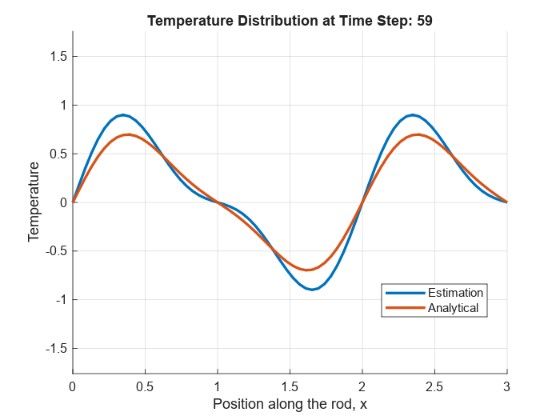
\includegraphics[width=0.8\textwidth]{heat_example.jpg}
    \caption{Iteration 59 of RK4 Solution to Heat Equation}
\end{figure}
With the proper function definition in MatLab, it is easy to use ode45() to obtain an equivalent solution. Note that for this comparison to work directly, the full vector of $t$ values used by RK4 was passed to ode45() as an input. This means that while ode45() is still free to adjust the step size as necessary, the outputted solution will be on the specified values. Shown below is an example plot of all three solutions on top of each other. To view the full solution animated, please run the main.m file and select the corresponding option.
\begin{figure}[H]
    \centering
    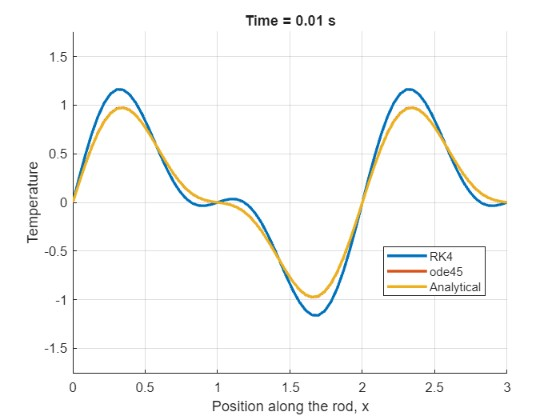
\includegraphics[width=0.8\textwidth]{heat_all_example.jpg}
    \caption{Iteration 34 of RK4 Solution and ode45() Solution vs. Analytical Solution to Heat Equation}
\end{figure}

\section{General Wave Equation}
\subsection*{$u_{tt} = 0.16u_{xx} + 0.02\sin(x+t)\\u(0,t) = 0.01\sin(t)\\u_x(2,t) = 0\\u(x,0) = \sin\left(\frac{\pi x}{2}\right)\\u_t(x,0) = \cos\left(\frac{\pi x}{2}\right)$}
Using the central difference approximation for second derivatives gives the following:
\begin{equation}
    \begin{aligned}
        &\frac{u_i^{n+1} - 2u_i^n + u_i^{n-1}}{\Delta t^2} = 0.16\left(\frac{u_{i+1}^n - 2u_i^n + u_{i-1}^n}{\Delta x^2}\right) + 0.02\sin\left(x+t\right)\\
        &u_i^{n+1} = \frac{0.16\Delta t^2}{\Delta x^2}\left(u_{i+1}^n - 2u_i^n + u_{i-1}^n\right) + 0.02\Delta t^2\sin\left(x+t\right) + 2u_i^n - u_i^{n-1}
    \end{aligned}
\end{equation}
Note that the $i$ index represents the spatial steps and the $n$ index represents the temporal steps. This gives a formulation for the next time step. Rewriting this gives a formulation for the current time step based on the previous time steps.
\begin{equation}
    u_i^{n} = \frac{0.16\Delta t^2}{\Delta x^2}\left(u_{i+1}^{n-1} - 2u_i^{n-1} + u_{i-1}^{n-1}\right) + 0.02\Delta t^2\sin\left(x+t\right) + 2u_i^{n-1} - u_i^{n-2}
\end{equation}
This is the form which will be implemented to produce the numerical solution. Note that this equation requires knowledge of the two previous time steps, and thus a different method is required for initialization. In order to do this, begin with the forward difference equation in time and the given initial condition.
\begin{equation}
    \frac{u_i^{n+1} - u_i^n}{\Delta t} = \cos\left(\frac{\pi x}{2}\right)
\end{equation}
For the wave equation, the other initial condition gives the value, but the wave equation requires two previous time steps. Using this formulation, a "ghost step" can be obtained and used to generate the first iteration of the wave equation. This is given by:
\begin{equation}
    u_i^0 = u_i^1 - \Delta t\cos\left(\frac{\pi x}{2}\right)
\end{equation}
For the boundary condition at the left endpoint, it is readily apparent that the formulation for this must be:
\begin{equation}
    u_{end}^n = u_{end-1}^n
\end{equation}
Shown below is an image of the wave at one of the iterations. To see the full animation, please run the main.m file and select the corresponding option.
\begin{figure}[H]
    \centering
    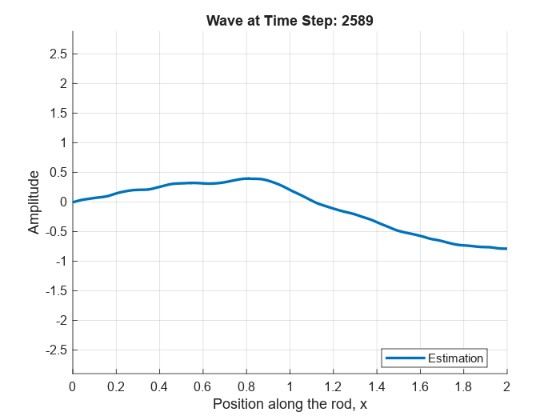
\includegraphics[width=0.8\textwidth]{wave_example.jpg}
    \caption{Iteration 2589 of Numerical Solution of Wave Equation}
\end{figure}

\section{Two-Dimensional General Heat Equation}
\subsection*{$u_t = 0.5\nabla^2u + e^{-t}u\\u_x(0,y,t) = 0\\u_y(x,0,t) = 0\\u(x,4,t) = e^{-t}\\u(4,y,t) = 0\\u(x,y,0) = \begin{cases}
1 & \text{for } y \geq x\\
0 & \text{for } y < x
\end{cases}$}
Using the forward difference approximation for first derivatives and the central difference approximation for second derivatives gives the following:
\begin{equation}
    \begin{aligned}
        &\frac{u_{i,j}^{n+1} - u_{i,j}^n}{\Delta t} = 0.5\left(\frac{u_{i+1,j}^n - 2u_{i,j}^n + u_{i-1,j}^n}{\Delta x^2} + \frac{u_{i,j+1}^n - 2u_{i,j}^n + u_{i,j-1}^n}{\Delta y^2}\right) + e^{-t}u_{i,j}^n\\
        &u_{i,j}^{n+1} = 0.5\Delta t\left(\frac{u_{i+1,j}^n - 2u_{i,j}^n + u_{i-1,j}^n}{\Delta x^2} + \frac{u_{i,j+1}^n - 2u_{i,j}^n + u_{i,j-1}^n}{\Delta y^2}\right) + \left(e^{-t}\Delta t + 1\right)u_{i,j}^n
    \end{aligned}
\end{equation}
In this case, $i$ and $j$ represent the $x$ and $y$ spatial steps, respectively. This gives a formulation for the next time step. Assuming the same step size for both spatial dimensions allows the simplificaiton $\Delta x = \Delta y = h$. Along with rewriting the formulation to give the current time step as a function of the previous time steps, this gives:
\begin{equation}
    u_{i,j}^n = \frac{0.5\Delta t}{h^2}\left(u_{i+1,j}^{n-1} + u_{i-1,j}^{n-1} + u_{i,j+1}^{n-1} + u_{i,j-1}^{n-1} - 4u_{i,j}^{n-1}\right) + \left(e^{-t}\Delta t + 1\right)u_{i,j}^{n-1}
\end{equation}
This is the form which will be implemented to produce the numerical solution. Similar to the wave equation above, for the derivative boundary conditions, it is readily apparent that the formulation for this must be:
\begin{equation}
    \begin{aligned}
        u_{start,j}^n = u_{start+1,j}^n\\
        u_{i,start}^n = u_{i,start+1}^n
    \end{aligned}
\end{equation}
Shown below is an image of the heat on the surface at one of the iterations. To see the full animation, please run the main.m file and select the corresponding option.
\begin{figure}[H]
    \centering
    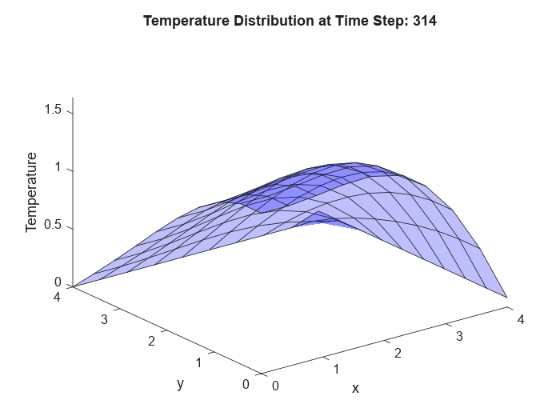
\includegraphics[width=0.8\textwidth]{2D_example.jpg}
    \caption{Iteration 314 of Numerical Solution of 2D Heat Equation}
\end{figure}

\section{Poisson's Equation}
\subsection*{$\nabla^2u = 1 + 0.2\delta_{(1,3)}(x,y) = f(x,y)\\u(x,4) = x\\u(2,y) = 1\\u(0,y) = 1 \text{ for } 2 \leq y \leq 4\\u(1,y) = 0 \text{ for } 0 \leq y \leq 2\\u(x,2) = 0 \text{ for } 0 \leq x \leq 1\\u(x,0) = 1 \text{ for } 1 \leq x \leq 2$}
Using the central difference approximation for the second derivatives gives:
\begin{equation}
    \left(\frac{u_{i+1,j}^n - 2u_{i,j}^n + u_{i-1,j}^n}{\Delta x^2} + \frac{u_{i,j+1}^n - 2u_{i,j}^n + u_{i,j-1}^n}{\Delta y^2}\right) = f(x,y)
\end{equation}
Assuming that $h=\Delta x=\Delta y$ gives:
\begin{equation}
    u_{i,j} = \frac{1}{4}\left(u_{i+1,j} + u_{i-1,j} + u_{i,j+1} + u_{i,j-1} - h^2f(x,y)\right)
\end{equation}
In order to solve this, use the method of iterative relaxation, where the matrix is initilized with zeros in all entries except the boundary conditions and iterations are performed until the change from step to step is within some specified tolerance. In some sense, this can be though of as iterating through the transient part of the 2D heat equation until the steady-state solution is achieved. Shown below is an image of the heat on the surface as determined by the iteration. To have a figure which can be manipulated in space, please run the main.m file and select the corresponding option.
\begin{figure}[H]
    \centering
    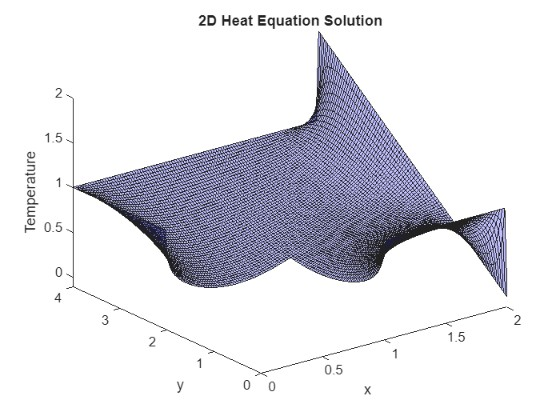
\includegraphics[width=0.8\textwidth]{poisson_example.jpg}
    \caption{Final Numerical Solution of Poisson's Equation}
\end{figure}

\section{Spacecraft Application}

\end{document}